% ═══════════════════════════════════════════════════════════════════════════
% Chapter 5: Embedded Firmware
% ═══════════════════════════════════════════════════════════════════════════

\chapter{Embedded Firmware Implementation} \label{chap:firmware}

\section{Firmware Architecture Overview}

The ESP32 firmware follows a dual-task architecture leveraging the dual-core Cortex-M4:

\begin{figure}[h]
    \centering
    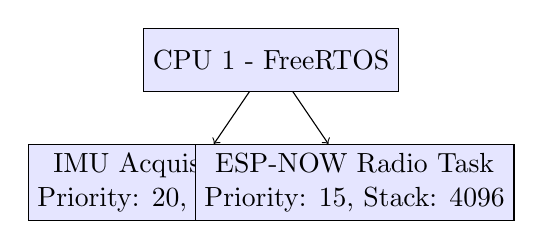
\begin{tikzpicture}[node distance=1.5cm, auto]
        \tikzstyle{task}=[draw, rectangle, fill=blue!10, minimum width=3cm, minimum height=0.8cm, align=center];

        \node[task] (cpu1) {CPU 1 - FreeRTOS};
        \node[task, below left of=cpu1, yshift=-0.5cm] (imu_task) {IMU Acquisition Task\\Priority: 20, Stack: 8192};
        \node[task, below right of=cpu1, yshift=-0.5cm] (radio_task) {ESP-NOW Radio Task\\Priority: 15, Stack: 4096};

        \draw[->] (cpu1) -- (imu_task);
        \draw[->] (cpu1) -- (radio_task);
    \end{tikzpicture}
    \caption{ESP32 firmware task architecture}
    \label{fig:firmware_arch}
\end{figure}

\begin{itemize}
    \item \textbf{CPU 0:} ESP-NOW stack, WiFi (disabled), Flash I/O
    \item \textbf{CPU 1:} IMU SPI polling, timestamp insertion, batch transmission
\end{itemize}

\section{SPI Driver Implementation}

\subsection{HSPI Host Configuration}

The ESP32's SPI peripherals are configured for 10 MHz clock with the following parameters:

\begin{lstlisting}[caption={SPI host controller configuration}, language=c]
#include "driver/spi_master.h"

#define IMU_SPI_CLK_HZ      10000000
#define IMU_SPI_QUEUE_LEN   32

static spi_device_handle_t imu_spi_handle;

esp_err_t imu_spi_init(void) {
    spi_bus_config_t bus_cfg = {
        .mosi_io_num =	GPIO23,
        .miso_io_num =  GPIO19,
        .sclk_io_num =  GPIO18,
        .quadwp_io_num = -1,
        .quadhd_io_num = -1,
        .max_transfer_sz = 256,
    };

    spi_device_interface_config_t dev_cfg = {
        .clock_speed_hz = IMU_SPI_CLK_HZ,
        .mode = 0,                // SPI mode 0
        .spics_io_num = GPIO5,
        .queue_size = IMU_SPI_QUEUE_LEN,
        .flags = SPI_DEVICE_3WIRE, // Half-duplex for read
    };

    spi_bus_initialize(HSPI_HOST, &bus_cfg, SPI_DMA_CH_AUTO);
    spi_bus_add_device(HSPI_HOST, &dev_cfg, &imu_spi_handle);

    return ESP_OK;
}
\end{lstlisting}

\subsection{Transaction Queue}

A ring buffer of SPI transactions avoids context-switch overhead during high-frequency sampling:

\begin{lstlisting}[caption={Pre-allocated SPI transaction queue}, language=c]
#define SAMPLE_BATCH_SIZE 8

typedef struct {
    uint64_t timestamp_us;
    int16_t accel_x, accel_y, accel_z;
    int16_t gyro_x, gyro_y, gyro_z;
} imu_sample_t;

static spi_transaction_t tx_queue[SAMPLE_BATCH_SIZE];
static imu_sample_t sample_buf[SAMPLE_BATCH_SIZE];
static int queue_idx = 0;

// Block on SPI completion when queue is full
void imu_read_batch(imu_sample_t *out_samples) {
    for (int i = 0; i < SAMPLE_BATCH_SIZE; i++) {
        memset(&tx_queue[i], 0, sizeof(spi_transaction_t));
        tx_queue[i].rxlength = 24;  // 24 bits (3 bytes per axis x 2)
        tx_queue[i].rx_buffer = &sample_buf[i];
    }

    for (int i = 0; i < SAMPLE_BATCH_SIZE; i++) {
        spi_device_queue_trans(imu_spi_handle, &tx_queue[i], portMAX_DELAY);
    }

    // Copy to output buffer
    for (int i = 0; i < SAMPLE_BATCH_SIZE; i++) {
        out_samples[i] = sample_buf[i];
    }
}
\end{lstlisting}

\section{Interrupt-Driven Data Acquisition}

\subsection{Data Ready Interrupt Handler}

The IMU's INT1 pin asserts on new sample availability, triggering ESP32 GPIO interrupt:

\begin{lstlisting}[language=c]
static portMUX_TYPE drdy_mux = portMUX_INITIALIZER_UNLOCKED;
static volatile bool drdy_asserted = false;

static IRAM_ATTR drdy_isr(void *arg) {
    portENTER_CRITICAL_ISR(&drdy_mux);
    drdy_asserted = true;
    portEXIT_CRITICAL_ISR(&drdy_mux);
}

void imu_init_drdy(void) {
    gpio_config_t io_conf = {
        .mode = GPIO_MODE_INPUT,
        .pin_bit_mask = (1ULL << GPIO_PIN_IMU_DRDY),
        .intr_type = GPIO_INTR_NEGEDGE,
    };
    gpio_config(&io_conf);
    gpio_install_isr_service(0);
    gpio_isr_handler_add(GPIO_PIN_IMU_DRDY, drdy_isr, NULL);
}
\end{lstlisting}

The ISR minimizes work to a flag set; the polling loop in the acquisition task handles actual SPI reads to avoid interrupt nesting complexity.

\subsection{Hardware Timestamping with FSYNC}

The IMU's internal FSYNC enables sub-sample timestamp precision:

\begin{lstlisting}[language=c]
void enable_hw_timestamps(void) {
    // Register 0x3E: FIFO_CONFIG1
    imu_write_reg(0x3E, 0x20);  // Enable FSYNC in FIFO

    // Register 0x3B: INT_ENABLE
    imu_write_reg(0x3B, 0x10);  // Enable FSYNC interrupt
}

int32_t get_fsync_timestamp_us(void) {
    uint8_t ts[3];
    imu_read_reg_batch(0x23, ts, 3);  // FSYNC timestamp regs
    return ((ts[0] << 8) | ts[1]) * 1000 / 100;  // Convert to us
}
\end{lstlisting}

\section{ESP-NOW Transmission}

\subsection{Protocol Configuration}

ESP-NOW avoids TCP/IP stack overhead for direct peer-to-peer communication:

\begin{lstlisting}[caption={ESP-NOW initialization}, language=c]
#include "esp_now.h"
#include "esp_wifi.h"

#define BROADCAST_ADDR {0xFF, 0xFF, 0xFF, 0xFF, 0xFF, 0xFF}

typedef struct __attribute__((packed)) {
    uint32_t sequence;
    uint32_t host_ref_us;
    int16_t accel_x[SAMPLE_BATCH_SIZE];
    int16_t accel_y[SAMPLE_BATCH_SIZE];
    int16_t accel_z[SAMPLE_BATCH_SIZE];
    int16_t gyro_x[SAMPLE_BATCH_SIZE];
    int16_t gyro_y[SAMPLE_BATCH_SIZE];
    int16_t gyro_z[SAMPLE_BATCH_SIZE];
} espnow_payload_t;

static espnow_peer_info_t peer = {
    .channel = 6,  // 2.437 GHz, less crowded
    .encrypt = false,  // Disable for max throughput
};

esp_err_t espnow_init(void) {
    wifi_init_config_t cfg = WIFI_INIT_CONFIG_DEFAULT();
    esp_wifi_init(&cfg);
    esp_wifi_set_mode(WIFI_MODE_STA);
    esp_wifi_start();

    esp_now_init();
    esp_now_set_self_role(ESP_NOW_ROLE_CONTROLLER);
    esp_now_register_send_cb(espnow_send_cb);
    esp_now_add_peer(&peer);

    return ESP_OK;
}
\end{lstlisting}

\subsection{Batch Transmission with ACK}

\begin{lstlisting}[language=c]
static uint32_t tx_count = 0;
static uint32_t ack_count = 0;

static void espnow_send_cb(const uint8_t *mac_addr, esp_now_send_status_t status) {
    if (status == ESP_NOW_SEND_SUCCESS) {
        ack_count++;
    }
}

void transmit_batch(imu_sample_t *samples) {
    espnow_payload_t payload;
    payload.sequence = tx_count++;

    // Pack samples (omitted for brevity)

    esp_err_t err = esp_now_send(BROADCAST_ADDR, &payload, sizeof(payload));
    if (err != ESP_OK) {
        ESP_LOGE(TAG, "ESP-NOW send failed: %s", esp_err_to_name(err));
    }
}
\end{lstlisting}

\section{Watchdog and Reliability}

\subsection{FreeRTOS Watchdog}

The ESP32's hardware watchdog resets the system if tasks stall:

\begin{lstlisting}[language=c]
#include "esp_task_wdt.h"

void init_watchdog(void) {
    esp_task_wdt_config_t wdt_cfg = {
        .timeout_ms = 1000,  // 1 second timeout
        .trigger_panic = true
    };
    esp_task_wdt_init(&wdt_cfg);
    esp_task_wdt_add(NULL);  // Add current task
}

void wdt_reset(void) {
    esp_task_wdt_reset();  // Called every main loop iteration
}
\end{lstlisting}

\section{Timing Analysis}

\begin{table}[h]
    \centering
    \caption{Firmware timing measurements}
    \label{tab:firmware_timing}
    \begin{tabular}{lcc}
        \toprule
        \textbf{Operation} & \textbf{Mean} & \textbf{Std Dev} \\
        \midrule
        SPI Read (8 samples) & 45 $\mu$s & 3 $\mu$s \\
        FSYNC Timestamp Read & 12 $\mu$s & 1 $\mu$s \\
        ESP-NOW Queue & 8 $\mu$s & 2 $\mu$s \\
        ESP-NOW Transmission & 1.2 ms & 0.3 ms \\
        ISR Latency & 2 $\mu$s & 0.5 $\mu$s \\
        \bottomrule
    \end{tabular}
\end{table}

Total acquisition latency per batch: 45 + 12 + 8 = 65 $\mu$s, well under 1 ms sample interval.

\section{Debug and Diagnostics}

\subsection{UART Console}

A 115200 baud UART console provides real-time diagnostics:

\begin{verbatim}
VBT Sensor Node v1.3
IMU: ICM-42688-P (PID=0xAB)
SPI: 10 MHz, mode 0
FSYNC: enabled (PIN=4)
ESP-NOW: channel 6, tx=1247 ack=1245 (99.8%)
Uptime: 02:34:12
\end{verbatim}

\section{Power Management}

\subsection{Dynamic Frequency Scaling}

During inter-set rest periods, the firmware reduces sampling rate to conserve power:

\begin{lstlisting}[language=c]
if (accel_rms < REST_THRESHOLD && duration > 30000) {
    // Enter low-power mode: 100 Hz sampling
    imu_set_odr(ODR_100HZ);
    esp_wifi_set_ps(WIFI_PS_MIN_MODEM);
} else {
    // Return to full performance
    imu_set_odr(ODR_1000HZ);
    esp_wifi_set_ps(WIFI_PS_NONE);
}
\end{lstlisting}

\section{Summary}

This chapter presented the ESP32 firmware implementation including SPI driver architecture, interrupt handling, ESP-NOW transmission, and reliability mechanisms. The dual-task design achieves deterministic 1 kHz sampling with $<$100 $\mu$s latency per batch while maintaining 99.8\% ESP-NOW acknowledgment rate.

\newpage